% ============================================================
%  Manuel d'Installation -- IoT Controller PWA
%  AOUAS Liza -- Master 1 EEA MTI -- Universite de Lorraine
%  Version amelioree v2.0 -- Juin 2026
% ============================================================
\documentclass[a4paper,12pt]{article}

% --- Encodage et langue ---
\usepackage[T1]{fontenc}
\usepackage[utf8]{inputenc}
\usepackage{times}
\usepackage{microtype}

% --- Mise en page ---
\usepackage[
  top=2.5cm, bottom=2.5cm,
  left=2.5cm, right=2.5cm,
  headheight=20pt
]{geometry}

% --- Couleurs ---
\usepackage[dvipsnames,table]{xcolor}
\definecolor{PrimaryBlue}{HTML}{1A3A5C}
\definecolor{AccentBlue}{HTML}{2E75B6}
\definecolor{LightBlue}{HTML}{D6E4F0}
\definecolor{SuccessGreen}{HTML}{1E7A3C}
\definecolor{LightGreen}{HTML}{D4EFDF}
\definecolor{WarnOrange}{HTML}{B8540A}
\definecolor{LightOrange}{HTML}{FAE5D3}
\definecolor{DangerRed}{HTML}{922B21}
\definecolor{LightRed}{HTML}{FADBD8}
\definecolor{TipPurple}{HTML}{6C3483}
\definecolor{LightPurple}{HTML}{EBD5F5}
\definecolor{CodeBg}{HTML}{F0F3F4}
\definecolor{TableHeader}{HTML}{2E75B6}
\definecolor{TableRowAlt}{HTML}{EBF5FB}
\definecolor{BorderGray}{HTML}{BDC3C7}
\definecolor{TextGray}{HTML}{5D6D7E}

% --- Boites colorees ---
\usepackage[most]{tcolorbox}
\tcbuselibrary{breakable,skins,listings}

% --- En-tetes et pieds de page ---
\usepackage{fancyhdr}
\usepackage{lastpage}

% --- Tableaux ---
\usepackage{tabularx}
\usepackage{booktabs}
\usepackage{multirow}
\usepackage{array}
\usepackage{colortbl}

% --- Listes ---
\usepackage{enumitem}

% --- Graphiques ---
\usepackage{graphicx}
\usepackage{amssymb}
\usepackage{tikz}
\usetikzlibrary{shapes.geometric,arrows.meta,positioning,fit,backgrounds,shadows.blur}

% --- Hyperliens ---
\usepackage{hyperref}
\hypersetup{
  colorlinks=true,
  linkcolor=AccentBlue,
  urlcolor=AccentBlue,
  pdftitle={Manuel d'Installation -- IoT Controller PWA},
  pdfauthor={AOUAS Liza},
}

% --- Code source ---
\usepackage{listings}
\lstdefinestyle{terminal}{
  backgroundcolor=\color{PrimaryBlue!95!black},
  basicstyle=\ttfamily\small\color{white},
  breaklines=true,
  frame=none,
  xleftmargin=12pt, xrightmargin=12pt,
  aboveskip=6pt, belowskip=6pt,
  keepspaces=true, showstringspaces=false,
}
\lstdefinestyle{code}{
  backgroundcolor=\color{CodeBg},
  basicstyle=\ttfamily\small\color{PrimaryBlue},
  breaklines=true,
  frame=leftline, framerule=3pt, rulecolor=\color{AccentBlue},
  xleftmargin=16pt, xrightmargin=8pt,
  aboveskip=6pt, belowskip=6pt,
  keepspaces=true, showstringspaces=false,
  commentstyle=\color{TextGray}\itshape,
}
\lstdefinestyle{output}{
  backgroundcolor=\color{LightGreen!50},
  basicstyle=\ttfamily\small\color{SuccessGreen!80!black},
  breaklines=true,
  frame=leftline, framerule=3pt, rulecolor=\color{SuccessGreen},
  xleftmargin=16pt, xrightmargin=8pt,
  aboveskip=4pt, belowskip=4pt,
  keepspaces=true, showstringspaces=false,
}

% ============================================================
%  BOITES PERSONNALISEES
% ============================================================
\tcbset{
  mybox/.style={
    enhanced, breakable,
    boxrule=0.8pt, arc=4pt,
    left=8pt, right=8pt, top=6pt, bottom=6pt,
    attach boxed title to top left={yshift=-2mm, xshift=8mm},
    boxed title style={arc=3pt, boxrule=0pt},
    fonttitle=\bfseries\small,
    before upper={\setlength{\parskip}{4pt}},
  },
}

\newcommand{\infobox}[2]{%
  \begin{tcolorbox}[mybox,
    colback=LightBlue, colframe=AccentBlue,
    colbacktitle=AccentBlue, coltitle=white,
    title={$\triangleright$\enspace #1}]#2\end{tcolorbox}}

\newcommand{\warnbox}[2]{%
  \begin{tcolorbox}[mybox,
    colback=LightOrange, colframe=WarnOrange,
    colbacktitle=WarnOrange, coltitle=white,
    title={$\triangle$\enspace #1}]#2\end{tcolorbox}}

\newcommand{\successbox}[2]{%
  \begin{tcolorbox}[mybox,
    colback=LightGreen, colframe=SuccessGreen,
    colbacktitle=SuccessGreen, coltitle=white,
    title={$\checkmark$\enspace #1}]#2\end{tcolorbox}}

\newcommand{\dangerbox}[2]{%
  \begin{tcolorbox}[mybox,
    colback=LightRed, colframe=DangerRed,
    colbacktitle=DangerRed, coltitle=white,
    title={$\times$\enspace #1}]#2\end{tcolorbox}}

\newcommand{\tipbox}[2]{%
  \begin{tcolorbox}[mybox,
    colback=LightPurple, colframe=TipPurple,
    colbacktitle=TipPurple, coltitle=white,
    title={$\star$\enspace #1}]#2\end{tcolorbox}}

% Etape numerotee
\newcommand{\etape}[2]{%
  \vspace{8pt}\noindent
  \begin{tikzpicture}[baseline=(num.base)]
    \node[circle, fill=AccentBlue, text=white,
          font=\bfseries\small, inner sep=4pt,
          minimum size=22pt] (num) {#1};
  \end{tikzpicture}
  \hspace{6pt}\textbf{#2}\par\vspace{2pt}}

% Commande inline
\newcommand{\cmd}[1]{\texttt{\colorbox{CodeBg}{\textcolor{PrimaryBlue}{#1}}}}

% ============================================================
%  EN-TETE ET PIED DE PAGE
% ============================================================
\pagestyle{fancy}
\fancyhf{}
\fancyhead[L]{\small\color{TextGray}\textbf{Manuel d'Installation} --- IoT Controller PWA}
\fancyhead[R]{\small\color{TextGray}AOUAS Liza --- Master 1 EEA MTI}
\fancyfoot[L]{\small\color{TextGray}Universit\'e de Lorraine --- UFR SFA}
\fancyfoot[C]{\small\color{TextGray}2025/2026}
\fancyfoot[R]{\small\color{TextGray}Page \thepage\ / \pageref{LastPage}}
\renewcommand{\headrulewidth}{1pt}
\renewcommand{\footrulewidth}{0.4pt}

% ============================================================
%  TITRES DE SECTIONS
% ============================================================
\usepackage{titlesec}
\newcommand{\sectionline}{{\color{AccentBlue}\titlerule[1.5pt]}}
\titleformat{\section}
  {\color{PrimaryBlue}\Large\bfseries}
  {\colorbox{AccentBlue}{\color{white}\enspace\thesection\enspace}}{10pt}{}
  [\sectionline]
\titleformat{\subsection}
  {\color{AccentBlue}\large\bfseries}
  {\thesubsection}{8pt}{}
\titleformat{\subsubsection}
  {\color{PrimaryBlue}\normalsize\bfseries}
  {\thesubsubsection}{6pt}{}
\titlespacing{\section}{0pt}{18pt}{10pt}
\titlespacing{\subsection}{0pt}{12pt}{6pt}

% ============================================================
\begin{document}

% ========================
%  PAGE DE GARDE
% ========================
\newgeometry{top=0cm,bottom=0cm,left=0cm,right=0cm}
\begin{titlepage}

\begin{tikzpicture}[remember picture, overlay]
  % Bande superieure - hauteur augmentee pour couvrir tout le texte d'en-tete
  \fill[PrimaryBlue] (current page.north west) rectangle
    ([yshift=-7.2cm] current page.north east);
  \fill[AccentBlue] ([yshift=-7.2cm] current page.north west) rectangle
    ([yshift=-7.55cm] current page.north east);
  % Bande inferieure
  \fill[PrimaryBlue] (current page.south west) rectangle
    ([yshift=2.2cm] current page.south east);
  \fill[AccentBlue] ([yshift=2.2cm] current page.south west) rectangle
    ([yshift=2.5cm] current page.south east);
\end{tikzpicture}
% Flush au bord superieur
\vspace*{1.4cm}
\begin{center}
  {\color{white}\Large\bfseries UNIVERSIT\'E DE LORRAINE}\\[4pt]
  {\color{white!85!PrimaryBlue}\normalsize Institut Sup\'erieur d'\'Electronique et d'Automatique (ISEA)}\\[2pt]
  {\color{white!85!PrimaryBlue}\normalsize UFR Sciences Fondamentales et Appliqu\'ees (SFA)}\\[2pt]
  {\color{white!85!PrimaryBlue}\normalsize Master 1 EEA --- Mesures et Traitement de l'Information (MTI)}\\[2pt]
  {\color{white!70!PrimaryBlue}\small Ann\'ee Universitaire 2025/2026}
\end{center}

\vspace{2.2cm}
\begin{center}
  {\color{TextGray}\small DOCUMENTATION TECHNIQUE}\\[8pt]
  \begin{tcolorbox}[
    enhanced, colback=white, colframe=AccentBlue,
    boxrule=2pt, arc=6pt,
    width=0.88\textwidth,
    halign=center, valign=center,
    left=16pt, right=16pt, top=14pt, bottom=14pt,
  ]
    {\color{PrimaryBlue}\Huge\bfseries Manuel d'Installation}\\[8pt]
    {\color{AccentBlue}\Large\bfseries IoT Controller --- Application PWA}\\[10pt]
    {\color{TextGray}\normalsize
    Guide complet d'installation sur PC Windows et Mobile\\[4pt]
    \texttt{ESP8266 + BMP280 + MQTT + Vue.js 3 + Node.js}}
  \end{tcolorbox}
\end{center}

\vspace{1.8cm}
\begin{center}
\begin{tcolorbox}[
  enhanced, colback=LightBlue!50, colframe=BorderGray,
  boxrule=0.8pt, arc=4pt, width=0.72\textwidth,
]
\renewcommand{\arraystretch}{1.5}
\begin{tabular}{@{}ll@{}}
  \textbf{\color{PrimaryBlue}Auteure :}        & Liza AOUAS \\
  \textbf{\color{PrimaryBlue}Encadrant :}      & M. Fabrice De Almeida Pereira Monteiro \\
  \textbf{\color{PrimaryBlue}Formation :}      & Master 1 EEA --- MTI \\
  \textbf{\color{PrimaryBlue}\'Etablissement :}& Universit\'e de Lorraine --- Metz \\
  \textbf{\color{PrimaryBlue}Ann\'ee :}        & 2025 -- 2026 \\
  \textbf{\color{PrimaryBlue}Version :}        & v2.0 --- Juin 2026 \\
\end{tabular}
\end{tcolorbox}
\end{center}

\vfill
\begin{center}
  {\color{white}\small Manuel d'Installation v2.0 --- Universit\'e de Lorraine --- 2025/2026}
\end{center}
\end{titlepage}
\restoregeometry

% ========================
%  TABLE DES MATIERES
% ========================
\thispagestyle{fancy}
\tableofcontents
\newpage

% ============================================================
\section{Introduction}
% ============================================================

Ce manuel d\'ecrit la proc\'edure compl\`ete d'installation de la plateforme de supervision IoT
\textbf{IoT Controller}. Il s'adresse \`a tout utilisateur souhaitant d\'eployer l'application
sur son environnement de travail, qu'il s'agisse d'un poste fixe sous Windows ou d'un
appareil mobile Android ou iOS.

\textbf{IoT Controller} est une \textbf{Progressive Web App (PWA)}, c'est-\`a-dire une
application web qui peut \^etre install\'ee sur le bureau ou l'\'ecran d'accueil et qui se comporte
comme une application native. Elle assure la supervision en temps r\'eel d'un \'equipement IoT
compos\'e d'un microcontr\^oleur ESP8266, d'un capteur BMP280 et d'un \'ecran OLED SSD1306.

\subsection*{Architecture du syst\`eme}

\vspace{10pt}
\begin{center}
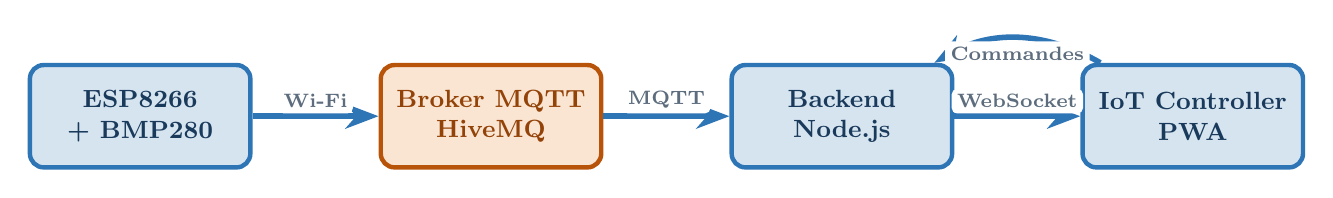
\begin{tikzpicture}[
  node distance=1.6cm,
  block/.style={
    rectangle, rounded corners=5pt,
    draw=AccentBlue, line width=1.6pt,
    fill=LightBlue, text=PrimaryBlue,
    font=\bfseries\small,
    minimum width=2.8cm, minimum height=1.3cm, align=center,
  },
  cloud/.style={
    block, fill=LightOrange, draw=WarnOrange, text=WarnOrange!80!black,
  },
  arrow/.style={-Stealth, line width=2pt, color=AccentBlue},
  lbl/.style={font=\scriptsize\bfseries, color=TextGray,
              fill=white, inner sep=2pt, rounded corners=2pt},
]
  \node[block] (esp)   {ESP8266\\+ BMP280};
  \node[cloud,  right=of esp]   (mqtt)  {Broker MQTT\\HiveMQ};
  \node[block,  right=of mqtt]  (back)  {Backend\\Node.js};
  \node[block,  right=of back]  (front) {IoT Controller\\PWA};

  \draw[arrow] (esp)  -- node[above,lbl]{Wi-Fi}    (mqtt);
  \draw[arrow] (mqtt) -- node[above,lbl]{MQTT}      (back);
  \draw[arrow] (back) -- node[above,lbl]{WebSocket} (front);
  \draw[arrow, bend right=30] (front) to node[below,lbl]{Commandes} (back);
\end{tikzpicture}
\end{center}
\vspace{6pt}

\infobox{Ordre de lecture recommand\'e}{
Suivez ce manuel dans l'ordre des sections. Chaque \'etape est un pr\'erequis de la suivante.
Ne sautez aucune section lors de la premi\`ere installation.
}

% ============================================================
\section{Pr\'erequis et configuration requise}
% ============================================================

\subsection{Configuration mat\'erielle minimale}

\renewcommand{\arraystretch}{1.3}
\begin{center}
\begin{tabular}{>{\bfseries\color{PrimaryBlue}}m{5cm} m{8.5cm}}
\rowcolor{TableHeader}
\multicolumn{1}{l}{\color{white}\bfseries \'El\'ement} &
\multicolumn{1}{l}{\color{white}\bfseries Configuration requise} \\
\rowcolor{white}       Syst\`eme d'exploitation & Windows 10 ou sup\'erieur (64 bits) \\
\rowcolor{TableRowAlt} Processeur               & Intel Core i3 ou \'equivalent (1,6 GHz minimum) \\
\rowcolor{white}       M\'emoire RAM            & 4 Go minimum (8 Go recommand\'e) \\
\rowcolor{TableRowAlt} Espace disque            & 500 Mo minimum pour les d\'ependances npm \\
\rowcolor{white}       Connexion r\'eseau       & Wi-Fi 2,4 GHz ou Ethernet \\
\rowcolor{TableRowAlt} Navigateur               & Microsoft Edge 90+ ou Google Chrome 90+ \\
\end{tabular}
\end{center}

\subsection{Logiciels \`a installer}

\begin{center}
\begin{tabular}{>{\bfseries\color{PrimaryBlue}}m{3.5cm} m{3cm} m{7cm}}
\rowcolor{TableHeader}
\multicolumn{1}{l}{\color{white}\bfseries Logiciel} &
\color{white}\bfseries Version &
\color{white}\bfseries Lien de t\'el\'echargement \\
\rowcolor{white}       Node.js      & 18.x ou sup. & \url{https://nodejs.org} \\
\rowcolor{TableRowAlt} Arduino IDE  & 2.x           & \url{https://www.arduino.cc/en/software} \\
\end{tabular}
\end{center}

\subsection{Composants mat\'eriels n\'ecessaires}

\begin{center}
\begin{tabular}{>{\bfseries\color{PrimaryBlue}}m{3.5cm} m{4cm} m{6cm}}
\rowcolor{TableHeader}
\multicolumn{1}{l}{\color{white}\bfseries Composant} &
\color{white}\bfseries R\'ef\'erence &
\color{white}\bfseries R\^ole \\
\rowcolor{white}       Microcontr\^oleur & NodeMCU ESP8266     & Acquisition et publication des donn\'ees \\
\rowcolor{TableRowAlt} Capteur           & BMP280 (I2C)        & Mesure de temp\'erature et de pression \\
\rowcolor{white}       Afficheur         & OLED SSD1306 128x64 & Affichage local des donn\'ees \\
\rowcolor{TableRowAlt} C\^able USB       & Micro-B vers USB-A  & Connexion PC pour le flash du firmware \\
\end{tabular}
\end{center}

\subsection{Configuration r\'eseau requise}

\warnbox{Ports r\'eseau \`a d\'ebloquer}{
V\'erifiez que ces ports ne sont pas bloqu\'es par votre pare-feu Windows avant de commencer~:
\begin{itemize}[noitemsep]
  \item \cmd{3000} --- Serveur backend Node.js (HTTP + WebSocket)
  \item \cmd{4173} --- Serveur frontend de production (\texttt{serve})
  \item \cmd{1883} --- Broker MQTT HiveMQ (TCP sortant vers internet)
\end{itemize}
Pour d\'esactiver temporairement le pare-feu~: \textbf{Param\`etres $\rightarrow$ S\'ecurit\'e Windows $\rightarrow$ Pare-feu $\rightarrow$ D\'esactiver}.
}

% ============================================================
\section{Installation de Node.js}
% ============================================================

Node.js est l'environnement d'ex\'ecution n\'ecessaire pour faire fonctionner le serveur backend.

\vspace{4pt}
\etape{1}{T\'el\'echargement de Node.js}
\begin{enumerate}[noitemsep, label=\alph*)]
  \item Ouvrez votre navigateur et acc\'edez \`a \url{https://nodejs.org}
  \item Cliquez sur le bouton vert \textbf{LTS (Long Term Support)}
  \item Attendez la fin du t\'el\'echargement --- fichier : \cmd{node-v18.x.x-x64.msi}
\end{enumerate}

\etape{2}{Installation de Node.js}
\begin{enumerate}[noitemsep, label=\alph*)]
  \item Double-cliquez sur le fichier \cmd{.msi} t\'el\'echarg\'e
  \item Cliquez \textbf{Next} \`a chaque \'ecran en laissant toutes les options par d\'efaut
  \item Cliquez \textbf{Install} puis \textbf{Finish}
\end{enumerate}

\etape{3}{V\'erification de l'installation}

Ouvrez un terminal \textbf{PowerShell} (\cmd{Win + R} puis tapez \cmd{powershell}) et saisissez~:

\begin{lstlisting}[style=terminal]
node --version
npm --version
\end{lstlisting}

R\'esultat attendu~:
\begin{lstlisting}[style=output]
v18.19.0
9.2.0
\end{lstlisting}

\successbox{Node.js install\'e avec succ\`es}{
Si les num\'eros de version s'affichent, Node.js est correctement install\'e. Vous pouvez passer \`a l'\'etape suivante.
}

% ============================================================
\section{Flash du firmware sur l'ESP8266}
% ============================================================

Cette \'etape consiste \`a programmer le microcontr\^oleur ESP8266 avec le firmware du projet.
Ce firmware permet de lire les donn\'ees du capteur BMP280, de les publier via MQTT et de
g\'erer l'\'ecran OLED.

\dangerbox{Conflit de port s\'erie --- \`A lire avant de commencer}{
Le backend Node.js et Arduino IDE \textbf{ne peuvent pas utiliser le port COM3 simultan\'ement}.
Si le backend est en cours d'ex\'ecution, arr\^etez-le avec \cmd{Ctrl + C} avant d'ouvrir Arduino IDE.
}

\etape{1}{Pr\'eparation d'Arduino IDE}
\begin{enumerate}[noitemsep, label=\alph*)]
  \item Ouvrez Arduino IDE
  \item Allez dans \textbf{Fichier $\rightarrow$ Ouvrir}
  \item Ouvrez : \cmd{MON\_PROJETS8/arduino\_export/arduino\_code.ino}
  \item \textbf{Outils $\rightarrow$ Type de carte} $\rightarrow$ s\'electionnez \cmd{NodeMCU 1.0 (ESP-12E Module)}
  \item \textbf{Outils $\rightarrow$ Port} $\rightarrow$ s\'electionnez le port disponible (ex: \cmd{COM3})
\end{enumerate}

\etape{2}{Configuration du r\'eseau Wi-Fi}

Dans \cmd{arduino\_code.ino}, modifiez les deux lignes suivantes~:

\begin{lstlisting}[style=code]
// Modifier avec vos identifiants Wi-Fi
const char* ssid     = "NOM_DE_VOTRE_WIFI";
const char* password = "MOT_DE_PASSE_WIFI";
\end{lstlisting}

\warnbox{Attention aux majuscules et \`a la bande Wi-Fi}{
Le SSID est \textbf{sensible \`a la casse}. L'ESP8266 est compatible \textbf{uniquement avec la bande 2,4 GHz} --- il ne peut pas se connecter \`a un r\'eseau 5 GHz.
}

\etape{3}{Upload du firmware}
\begin{enumerate}[noitemsep, label=\alph*)]
  \item Branchez l'ESP8266 \`a votre ordinateur via le c\^able USB
  \item Dans Arduino IDE, cliquez sur la fl\`eche \textbf{($\rightarrow$)} pour lancer l'upload
  \item Attendez environ 30 secondes jusqu'\`a voir : \cmd{Done uploading}
\end{enumerate}

\etape{4}{V\'erification via le Moniteur s\'erie}
\begin{enumerate}[noitemsep, label=\alph*)]
  \item Allez dans \textbf{Outils $\rightarrow$ Moniteur s\'erie}, vitesse \cmd{9600 baud}
  \item Vous devez voir~:
\end{enumerate}

\begin{lstlisting}[style=output]
BMP280 detecte OK !
WiFi connecte !
192.168.X.X
MQTT OK
Commandes actives
Metadata OK
\end{lstlisting}

\successbox{Firmware install\'e avec succ\`es}{
L'ESP8266 va maintenant automatiquement~:
\begin{itemize}[noitemsep]
  \item[$\checkmark$] Se connecter au Wi-Fi au d\'emarrage
  \item[$\checkmark$] Se connecter au broker MQTT HiveMQ
  \item[$\checkmark$] Publier ses m\'etadonn\'ees (description des capteurs)
  \item[$\checkmark$] Envoyer les mesures toutes les 5 secondes
\end{itemize}
}

% ============================================================
\section{Installation et d\'emarrage du backend}
% ============================================================

Le backend est un serveur Node.js qui fait le lien entre le broker MQTT et l'interface web.
Il re\c{c}oit les donn\'ees de l'ESP8266 et les redistribue en temps r\'eel via WebSocket.

\etape{1}{Installation des d\'ependances}

Fermez compl\`etement Arduino IDE. Ouvrez un terminal \textbf{PowerShell}~:

\begin{lstlisting}[style=terminal]
cd C:\Users\...\mon_projets8\backend
npm install
\end{lstlisting}

\etape{2}{V\'erification du fichier de configuration}

V\'erifiez que le fichier \cmd{.env} contient~:

\begin{lstlisting}[style=code]
PORT=3000
MQTT_BROKER=mqtt://broker.hivemq.com
SERIAL_PORT=COM3
SERIAL_BAUD=9600
\end{lstlisting}

\etape{3}{D\'emarrage du backend}

\begin{lstlisting}[style=terminal]
node server.js
\end{lstlisting}

R\'esultat attendu dans le terminal~:

\begin{lstlisting}[style=output]
Serveur demarre sur http://localhost:3000
Connecte au broker MQTT
Abonne au topic : +/datalog/+/+
Abonne au topic : +/metadata/flows
Metadata recue depuis : ESP8266_Liza
temperature, pression
\end{lstlisting}

\dangerbox{Ne pas fermer ce terminal}{
Le terminal du backend \textbf{doit rester ouvert} pendant toute la dur\'ee d'utilisation.
Fermer ce terminal entra\^ine la d\'econnexion de l'interface web.
}

\tipbox{Astuce : diagnostic MQTT}{
Si \texttt{Connecte au broker MQTT} n'appara\^it pas apr\`es 10 secondes, v\'erifiez votre connexion internet et que le port \cmd{1883} (TCP sortant) n'est pas bloqu\'e par un pare-feu ou un proxy.
}

% ============================================================
\section{Build et d\'emarrage du frontend}
% ============================================================

\infobox{Mode production vs mode d\'eveloppement}{
Contrairement \`a \cmd{npm run dev} (port 5173), le mode production g\'en\`ere le \textbf{Service Worker PWA} qui permet l'installation en tant qu'application native et le fonctionnement hors-ligne.
}

\etape{1}{Installation des d\'ependances frontend}

Ouvrez un \textbf{nouveau terminal} (laissez le backend ouvert)~:

\begin{lstlisting}[style=terminal]
cd C:\Users\...\mon_projets8\frontend
npm install
\end{lstlisting}

\etape{2}{Build de production}

\begin{lstlisting}[style=terminal]
npm run build
\end{lstlisting}

R\'esultat attendu \`a la fin du build~:

\begin{lstlisting}[style=output]
built in XX.XXs

PWA v1.3.0
mode       generateSW
precache   5 entries
files generated
  dist/sw.js
  dist/workbox-XXXXX.js
\end{lstlisting}

\successbox{Build r\'eussi}{
La pr\'esence de \cmd{dist/sw.js} confirme que la PWA est correctement configur\'ee et pr\^ete pour l'installation.
}

\etape{3}{Installation du serveur de production}

\begin{lstlisting}[style=terminal]
npm install -g serve
\end{lstlisting}

\etape{4}{Lancement du serveur frontend}

\begin{lstlisting}[style=terminal]
serve -s dist -l 4173
\end{lstlisting}

R\'esultat attendu~:

\begin{lstlisting}[style=output]
Serving!

  - Local   :  http://localhost:4173
  - Network :  http://192.168.X.X:4173
\end{lstlisting}

\warnbox{Notez l'adresse Network}{
L'adresse \cmd{http://192.168.X.X:4173} est indispensable pour l'installation de la PWA sur mobile. Notez-la maintenant.
}

% ============================================================
\section{Installation de la PWA sur PC Windows}
% ============================================================

Une PWA install\'ee se comporte comme une application Windows native : ic\^one sur le bureau,
fen\^etre propre sans barre d'adresse, pr\'esence dans le menu D\'emarrer.

\begin{center}
\begin{tcolorbox}[
  enhanced, colback=LightBlue!30, colframe=AccentBlue,
  boxrule=0.8pt, arc=4pt, width=0.88\textwidth,
]
\textbf{\color{PrimaryBlue}Avantages de l'installation PWA}

\vspace{4pt}
\begin{tabular}{@{\quad$\checkmark$\enspace}l}
  Lancement rapide depuis le bureau sans ouvrir le navigateur \\
  Fen\^etre propre sans la barre d'adresse du navigateur \\
  Ic\^one personnalis\'ee dans la barre des t\^aches \\
  Fonctionnement partiel hors-ligne gr\^ace au Service Worker \\
  Mise \`a jour automatique lors de la prochaine connexion \\
\end{tabular}
\end{tcolorbox}
\end{center}

\etape{1}{Ouverture dans Microsoft Edge}
\begin{enumerate}[noitemsep, label=\alph*)]
  \item Ouvrez Microsoft Edge
  \item Dans la barre d'adresse, tapez : \cmd{http://localhost:4173}
  \item Appuyez sur Entr\'ee et attendez que le dashboard se charge compl\`etement
\end{enumerate}

\etape{2}{Lancement de l'installation}

\vspace{4pt}\noindent\textbf{M\'ethode A --- Via la barre d'adresse (recommand\'ee)~:}
\begin{enumerate}[noitemsep, label=\alph*)]
  \item Regardez la barre d'adresse en haut de Edge
  \item Cliquez sur l'ic\^one en forme d'\'ecran avec un \textbf{+}
  \item Cliquez \textbf{Installer} dans la fen\^etre qui appara\^it
\end{enumerate}

\vspace{4pt}\noindent\textbf{M\'ethode B --- Via le menu Edge~:}
\begin{enumerate}[noitemsep, label=\alph*)]
  \item Cliquez sur les 3 points \textbf{(\ldots)} en haut \`a droite
  \item \textbf{Applications $\rightarrow$ Installer IoT Controller}
  \item Cliquez \textbf{Installer}
\end{enumerate}

\successbox{Installation PC r\'eussie --- V\'erifications}{
\begin{itemize}[noitemsep]
  \item[$\checkmark$] Une ic\^one \textbf{IoT Controller} est apparue sur votre bureau
  \item[$\checkmark$] L'application s'est ouverte dans sa propre fen\^etre
  \item[$\checkmark$] La barre de navigation d'Edge n'est plus visible
  \item[$\checkmark$] L'application appara\^it dans le menu D\'emarrer de Windows
\end{itemize}
}

% ============================================================
\section{Installation de la PWA sur mobile}
% ============================================================

\infobox{Condition requise}{
Votre t\'el\'ephone mobile doit \^etre connect\'e au \textbf{m\^eme r\'eseau Wi-Fi} que l'ordinateur.
Utilisez l'adresse \cmd{http://192.168.X.X:4173} affich\'ee au d\'emarrage du serveur frontend.
}

\subsection{Installation sur Android}

\etape{1}{Ouvrir dans Chrome}
\begin{enumerate}[noitemsep, label=\alph*)]
  \item Connectez votre t\'el\'ephone Android au m\^eme r\'eseau Wi-Fi
  \item Ouvrez \textbf{Google Chrome} et tapez l'adresse r\'eseau : \cmd{http://192.168.X.X:4173}
\end{enumerate}

\etape{2}{Installer l'application}
\begin{enumerate}[noitemsep, label=\alph*)]
  \item Une banni\`ere appara\^it en bas : \textit{Ajouter IoT Controller \`a l'\'ecran d'accueil}
  \item Appuyez sur la banni\`ere, puis sur \textbf{Ajouter}
\end{enumerate}

\tipbox{Si la banni\`ere n'appara\^it pas}{
Appuyez sur les 3 points en haut \`a droite de Chrome, puis sur \textbf{Ajouter \`a l'\'ecran d'accueil} et confirmez.
}

\subsection{Installation sur iOS (iPhone)}

\warnbox{Safari uniquement sur iOS}{
L'installation PWA sur iOS fonctionne \textbf{uniquement avec Safari}. Chrome sur iOS ne permet pas l'installation native.
}

\begin{enumerate}[noitemsep, label=\alph*)]
  \item Connectez votre iPhone au m\^eme r\'eseau Wi-Fi
  \item Ouvrez \textbf{Safari} et tapez : \cmd{http://192.168.X.X:4173}
  \item Appuyez sur l'ic\^one \textbf{Partager} (carr\'e avec fl\`eche vers le haut)
  \item Dans le menu, appuyez sur \textbf{Sur l'\'ecran d'accueil}
  \item Confirmez en appuyant sur \textbf{Ajouter}
\end{enumerate}

% ============================================================
\section{Proc\'edure de d\'emarrage compl\`ete}
% ============================================================

Chaque fois que vous utilisez IoT Controller, respectez cet ordre~:

\vspace{6pt}
\renewcommand{\arraystretch}{1.4}
\begin{center}
\begin{tabular}{>{\centering\bfseries\color{white}}m{1cm}
                >{\bfseries\color{PrimaryBlue}}m{4.5cm}
                m{8cm}}
\rowcolor{TableHeader}
\color{white}\# & \color{white}Action & \color{white}D\'etails et commande \\
\rowcolor{white}       1 & Fermer Arduino IDE   & Lib\'erer le port COM3 \\
\rowcolor{TableRowAlt} 2 & Brancher l'ESP8266   & C\^able USB entre l'ESP8266 et le PC \\
\rowcolor{white}       3 & D\'emarrer le backend & \cmd{cd backend \&\& node server.js} \\
\rowcolor{TableRowAlt} 4 & D\'emarrer le frontend & \cmd{cd frontend \&\& serve -s dist -l 4173} \\
\rowcolor{white}       5 & Ouvrir l'application & Double-cliquer sur l'ic\^one IoT Controller \\
\end{tabular}
\end{center}

\vspace{8pt}
\successbox{V\'erification du bon d\'emarrage}{
Contr\^olez ces points dans la barre de statut apr\`es l'ouverture~:
\begin{itemize}[noitemsep]
  \item[$\checkmark$] \textbf{Backend :} Connect\'e (indicateur vert)
  \item[$\checkmark$] \textbf{MQTT :} Actif (indicateur vert)
  \item[$\checkmark$] \textbf{ESP8266\_Liza} affich\'e comme appareil connect\'e
  \item[$\checkmark$] Badge \textbf{LIVE} clignotant en vert dans le header
  \item[$\checkmark$] Valeurs de temp\'erature et pression mises \`a jour toutes les 5 secondes
\end{itemize}
}

% ============================================================
\section{R\'esolution des probl\`emes fr\'equents}
% ============================================================

\renewcommand{\arraystretch}{1.4}
\begin{center}
\begin{tabular}{>{\bfseries\small\color{DangerRed}}m{5.5cm}
                >{\small}m{8.5cm}}
\rowcolor{TableHeader}
\multicolumn{1}{l}{\color{white}\bfseries Probl\`eme observ\'e} &
\multicolumn{1}{l}{\color{white}\bfseries Solution recommand\'ee} \\
\rowcolor{white}
\texttt{COM3 Access denied} au d\'emarrage &
Fermer compl\`etement Arduino IDE avant de lancer \cmd{node server.js} \\
\rowcolor{TableRowAlt}
Ic\^one PWA non visible dans Edge &
Utiliser \cmd{serve -s dist} (port 4173) et non \cmd{npm run dev} (port 5173) \\
\rowcolor{white}
Ancienne interface apr\`es un build &
Supprimer le dossier \cmd{dist/} et relancer \cmd{npm run build} \\
\rowcolor{TableRowAlt}
Le mobile ne trouve pas le serveur &
V\'erifier le m\^eme r\'eseau Wi-Fi, d\'esactiver temporairement le pare-feu Windows \\
\rowcolor{white}
Bandeau rouge hors-ligne &
D\'emarrer le backend avant l'application. V\'erifier \cmd{node server.js} \\
\rowcolor{TableRowAlt}
ESP8266 ne se connecte pas au Wi-Fi &
V\'erifier le SSID et le mot de passe. Le r\'eseau doit \^etre en 2,4 GHz \\
\rowcolor{white}
Pas de donn\'ees dans le graphique &
V\'erifier l'ESP8266 aliment\'e et connect\'e. Envoyer la commande \cmd{DESCRIBE} \\
\rowcolor{TableRowAlt}
MQTT non joignable &
V\'erifier la connexion internet et le port 1883 (TCP sortant) \\
\rowcolor{white}
M\'etadonn\'ees jamais re\c{c}ues &
Envoyer la commande \cmd{DESCRIBE} depuis le dashboard pour forcer la republication \\
\end{tabular}
\end{center}

\begin{tcolorbox}[mybox,
    colback=LightPurple, colframe=TipPurple,
    colbacktitle=TipPurple, coltitle=white,
    title={$\star$\enspace Diagnostic r\'eseau rapide}]
Pour tester la connectivit\'e backend depuis le navigateur, ouvrez la console (F12) et tapez~:

\medskip
\begin{minipage}{\linewidth}
\colorbox{CodeBg}{%
  \begin{minipage}{0.96\linewidth}
  \vspace{4pt}
  {\ttfamily\small\color{PrimaryBlue}%
  fetch('http://localhost:3000')\\
  \hspace*{12pt}.then(r => console.log('Backend OK :', r.status))\\
  \hspace*{12pt}.catch(e => console.error('Injoignable :', e));%
  }
  \vspace{4pt}
  \end{minipage}%
}
\end{minipage}
\end{tcolorbox}

% ============================================================
\section{Glossaire}
% ============================================================

\renewcommand{\arraystretch}{1.4}
\begin{center}
\begin{tabular}{>{\bfseries\color{AccentBlue}}m{3.5cm} m{10.5cm}}
\rowcolor{TableHeader}
\multicolumn{1}{l}{\color{white}\bfseries Terme} &
\multicolumn{1}{l}{\color{white}\bfseries D\'efinition} \\
\rowcolor{white}       ESP8266 & Microcontr\^oleur Wi-Fi d'Espressif, passerelle IoT du projet \\
\rowcolor{TableRowAlt} BMP280  & Capteur barom\'etrique Bosch (temp\'erature + pression), bus I2C \\
\rowcolor{white}       MQTT    & Protocole de messagerie l\'eger pub/sub, standard de l'IoT \\
\rowcolor{TableRowAlt} HiveMQ  & Broker MQTT public utilis\'e comme relais de messages \\
\rowcolor{white}       Node.js & Environnement d'ex\'ecution JavaScript c\^ot\'e serveur \\
\rowcolor{TableRowAlt} Socket.IO & Communication temps r\'eel bidirectionnelle (WebSocket) \\
\rowcolor{white}       PWA     & Progressive Web App~: application web installable nativement \\
\rowcolor{TableRowAlt} Service Worker & Script de cache et de mode hors-ligne de la PWA \\
\rowcolor{white}       RETAIN  & Flag MQTT~: le broker conserve et renvoie le dernier message \\
\rowcolor{TableRowAlt} Vue.js  & Framework JavaScript utilis\'e pour le dashboard \\
\end{tabular}
\end{center}

\vspace{16pt}
\begin{center}
  \color{TextGray}\small
  \textit{Manuel d'Installation v2.0 --- IoT Controller PWA --- AOUAS Liza}\\
  \textit{Master 1 EEA MTI --- Universit\'e de Lorraine --- UFR SFA --- 2025/2026}
\end{center}

\end{document}